%%%%%%%%%%%%%%%%%%%%%%%%%%%%%%%%%%%%%%%%%%%
\section{Plant Physiology}
%%%%%%%%%%%%%%%%%%%%%%%%%%%%%%%%%%%%%%%%%%%
A plant's health is greatly determined by the availability of light, water, and key nutrients in the soil.  These elements are the fundamental inputs to photosynthesis, the process plants utilize to turn light energy into chemical energy for growth.  Nitrogen, Potassium, and Phosphorus are fertilizers (agricultural inputs) that can incur large costs when applied over hectares of farmland, but are needed for healthy plant growth and cell reproduction.

Water is also an essential agricultural input needed for plant photosynthesis and aids in nutrient transport.  Droughts are becoming a global epidemic and precision water management is becoming pivotal for a crops' survival.

The layers of a deciduous leaf contain protection mechanisms, transport systems, and reaction centers for the process of photosynthesis.
%
\begin{figure}[!htb]
    \begin{center}
        \makebox[\textwidth]{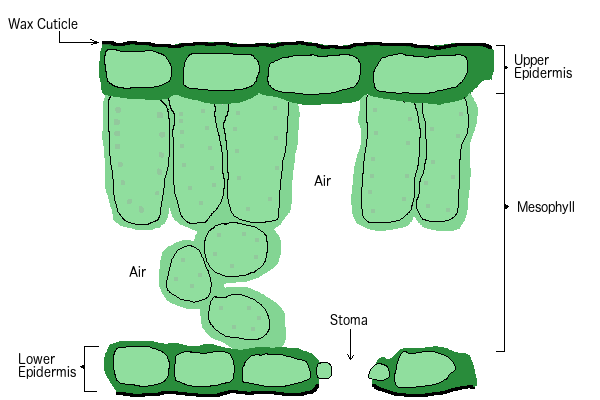
\includegraphics[scale=0.5]{/Sources/Background/Plant_Physiology/leaf-v3.png}}
    \end{center}
    \caption{Major Structures of a Leaf}
    \label{fig:polarization}
\end{figure}
%
The cuticle wax layer, upper epidermis, and mesophyll layer are the first layers of light interaction on the adaxial surface of the leaf.

The cuticle wax layer provides “the most critical adaptive trait for survival … the ability to retain water in increasingly dehydrating habitats” \cite{cuticle}.  It is the first line of defense for plants and acts as a barrier between water transpiration.

The mesophyll layers contain chloroplasts that convert light energy into chemical energy and consists of two parts. The palisade mesophyll is made up of elongated, organized, compact cells that contain a large number of the chloroplasts.  The spongy mesophyll is irregular in shape and has a large amount of space between its cells to facilitate air and gas exchange \cite{plantexchange}.

The upper epidermis consists of very few chloroplasts, and allows most of the light to pass through to the mesophyll layers.


%%%%%%%%%%%%%%%%%%%%%%%%%%%%%%%%%%%%%%%%%%%
\subsection{Photosynthesis}
%%%%%%%%%%%%%%%%%%%%%%%%%%%%%%%%%%%%%%%%%%%

Photosynthesis is a fundamental process that dictates the growth of all land plants.  Water plays an important role in this chemical process, and its availability in plant leaves is an indicator of the plant's ability to perform photosynthesis.

The chemical reaction undergone during photosynthesis involves the conversion of carbon dioxide and water with light energy, to create a carbohydrate and oxygen.  It is formally written as,
%
\begin{align}
    6CO_2 + 6H_2O \xrightarrow{\text{light}} C_6H_12O_6 + 6O_2
\end{align}
%
Due to water's integral role in this reaction, water stress in plants can lead to decreased photosynthetic activity.  It was pointed out by Ehleringer, referenced in \cite{akinci}, that water stress “can decrease…photosynthesis by reflecting quanta that might have been used in photosynthesis”.   Chlorophyll is an essential pigment in photosynthesis due to it being “an efficient light-absorbing molecule” \cite{ecophysiology}.  It is highly absorbing in the blue and red spectrum of visible light, and more reflective in the green portion.  The absorption spectrum for chlorophyll can be found in \cite{chemistry}. This spectrum is what causes many leaves to appear green.  Note that is regions outside the visible, chlorophyll does not absorb the incident radiation.

%%%%%%%%%%%%%%%%%%%%%%%%%%%%%%%%%%%%%%%%%%%
\subsection{Relative Water Content}
%%%%%%%%%%%%%%%%%%%%%%%%%%%%%%%%%%%%%%%%%%%
The Relative Water Content (RWC) of a leaf is a measure of the current water level based on the total leaf water retaining capacity.  It is a useful measure of the water balance within a plant as it expresses the absolute amount of current water in a plant, in proportion to the minimum amount of water it can hold.

Water makes up over 90\% of the mass of a leaf, and although RWC provides a good indicator of plant health and water capacity, it is highly dependent on the age and maturity of the leaf.  It should also be taken into consideration that leaves can also be very heterogeneous and contain a variety of complex structures in different stages of growth, within each individual leaf.

Correlations between the RWC and other physiological responses have been found in [9].

\begin{table}[h]
  \centering
  \begin{tabular}{ll}
    \toprule
    \textbf{Relative Water Content ~(\%)}      & \textbf{Plant Physiological Response}\\
    \midrule
      \texttt{90-100}          & closing of the stomata, reduction of cellular expansion and growth\\
      \texttt{80-90}           & tissue composition change, altered rates of photosynthesis and respiration\\
      \texttt{<80}         & ceasing of photosynthesis\\
    \bottomrule
  \end{tabular}
  \caption{%
    Plant physiological responses to detected relative water content levels.
  }
  \label{tab:Packages}
\end{table}

“An increase in reflectance…is not directly related to water content but indirectly, since a decrease in water content can lead to an increase in internal lead air space or cell breakdown which may increase reflectance and decrease transmittance [2]”.

This increase in internal air space leads to multiple scattering at air wax boundaries, and creates differences in the reflection and transmission of light, absorption, and the $S1$ and $S2$ Stokes parameters of the polarization response.

Field measurements of the physiological properties of plants are time consuming and error prone.  It is therefore beneficial to pursue solutions to quantifying these metrics in large area field measurements.

